\chapter{The Wu Pipeline, Step by Step}
\label{chap:wu_pipeline}

This chapter walks through the executable steps in \texttt{wu/steps/}
that take the raw Fortran output to the piecewise diagnostics.  Each
step is illustrated with the figure it generates (regenerated for this
handbook into \texttt{handbook/figs/wu/}).

\section{Step 05 --- Pass A/B: PV, Boundary \texorpdfstring{$\theta$}{theta}, Balanced \texorpdfstring{$\psi$}{psi}}
\label{sec:step05}

Step~05 compiles the three Fortran programs and runs \texttt{pvpialln}
twice: Pass~A on the 30-year mean state (\texttt{meanq}, \texttt{meanh})
and Pass~B on the 2025-01-08 event state (\texttt{event\_q.out},
\texttt{event\_h.out}).  It computes the boundary $\theta$
($\theta_b^{\text{bot}}$ at 1000, $\theta_b^{\text{top}}$ at 100\,hPa),
the interior Ertel PV on $850$--$200$\,hPa, and the balanced
streamfunction.

\begin{figure}[H]
  \centering
  
\includegraphics[width=\textwidth]{figs/wu/wu_mean_pv_3levels.png}
  \caption[Pass A mean Ertel PV]{\textbf{Step 05 / Pass A.} Mean-state
  Ertel PV (Wu internal units) at three representative \emph{interior}
  levels.  The upper-level panel shows the climatological jet PV gradient
  that the event anomaly perturbs.}
  \label{fig:wu_mean_pv}
\end{figure}

\begin{figure}[H]
  \centering
  
\includegraphics[width=\textwidth]{figs/wu/wu_pv_anomaly_3levels.png}
  \caption[Event PV anomaly]{\textbf{Step 05 / Pass B.} Event-minus-mean
  PV anomaly $\dq$.  The dominant upper-tropospheric positive anomaly is
  the blocking ridge inverted in the \emph{upper} piece of Pass~D; the
  weak low-level anomaly is dwarfed by it (and the surface heating itself
  lives in the boundary $\theta$, not in this interior field).}
  \label{fig:wu_pv_anom}
\end{figure}

\begin{figure}[H]
  \centering
  
\includegraphics[width=0.78\textwidth]{figs/wu/wu_mean_psi_500hpa.png}
  \caption[Balanced mean streamfunction]{\textbf{Step 05.} Balanced
  mean-state streamfunction $\bpsi$ at $500$\,hPa --- the basic state
  about which the nonlinear (\texttt{INLIN}=1) perturbation inversion is
  linearised.}
  \label{fig:wu_mean_psi}
\end{figure}

\section{Step 06 --- Pass C: Total Balanced Inversion (BALNC)}
\label{sec:step06}

Step~06 runs \texttt{qinvert21} (BALNC) to produce the total balanced
$(\psi,\Phi)$ pair (\texttt{event\_bal.out}), the reference from which
Pass~D forms the perturbation.  Per-cycle convergence is reached
($\sim 10^{-4}$, below threshold); the trailing ``started diverging''
message is the benign outer-coupling heuristic of
\Cref{sec:wu_converge}, and the written field is the converged state.

\begin{figure}[H]
  \centering
  
\includegraphics[width=\textwidth]{figs/wu/pass_c_psi_all_levels.png}
  \caption[Pass C all levels]{\textbf{Step 06 / Pass C.} Total balanced
  streamfunction at all nine pressure levels, showing the
  equivalent-barotropic vertical structure of the blocking circulation.}
  \label{fig:wu_passc_all}
\end{figure}

\section{Step 07 --- Pass D: Piecewise Perturbation Inversion (BALP)}
\label{sec:step07}

Step~07 runs \texttt{qinvertp21} (BALP), partitioning $\dq$ into the
\textbf{surface}, \textbf{lower} and \textbf{upper} pieces
(\Cref{sec:wu_passes}) and inverting each to its perturbation
streamfunction $\psi'$.  All three report \texttt{TOTAL CONVERGENCE}.

\begin{figure}[H]
  \centering
  
\includegraphics[width=\textwidth]{figs/wu/pass_d_psi_3pieces_250hpa.png}
  \caption[Pass D three pieces]{\textbf{Step 07 / Pass D.} $250$\,hPa
  perturbation streamfunction $\psi'$ induced by each piece:
  \textbf{(a)} surface ($1000$\,hPa boundary $\theta$),
  \textbf{(b)} lower ($850$--$700$\,hPa PV),
  \textbf{(c)} upper ($500$--$200$\,hPa PV $+$ $100$\,hPa top $\theta$).
  The upper piece dominates the jet-level response; the surface piece is
  a broad, predominantly cyclonic ($\psi'<0$) response to the net-warm
  surface $\theta'$.}
  \label{fig:wu_passd_3}
\end{figure}

\section{Step 08 --- Wu \texorpdfstring{$Q$}{Q} vs ERA5 Ertel PV}
\label{sec:step08}

Step~08 parses all Fortran outputs, converts Wu $Q$ to SI by the exact
$10^{-8}$ constant (\Cref{chap:wu_coeffs}), and computes the induced
winds and PV advection, writing \texttt{piecewise\_psi.nc} and
\texttt{pv\_advection.nc} (all SI).

\begin{figure}[H]
  \centering
  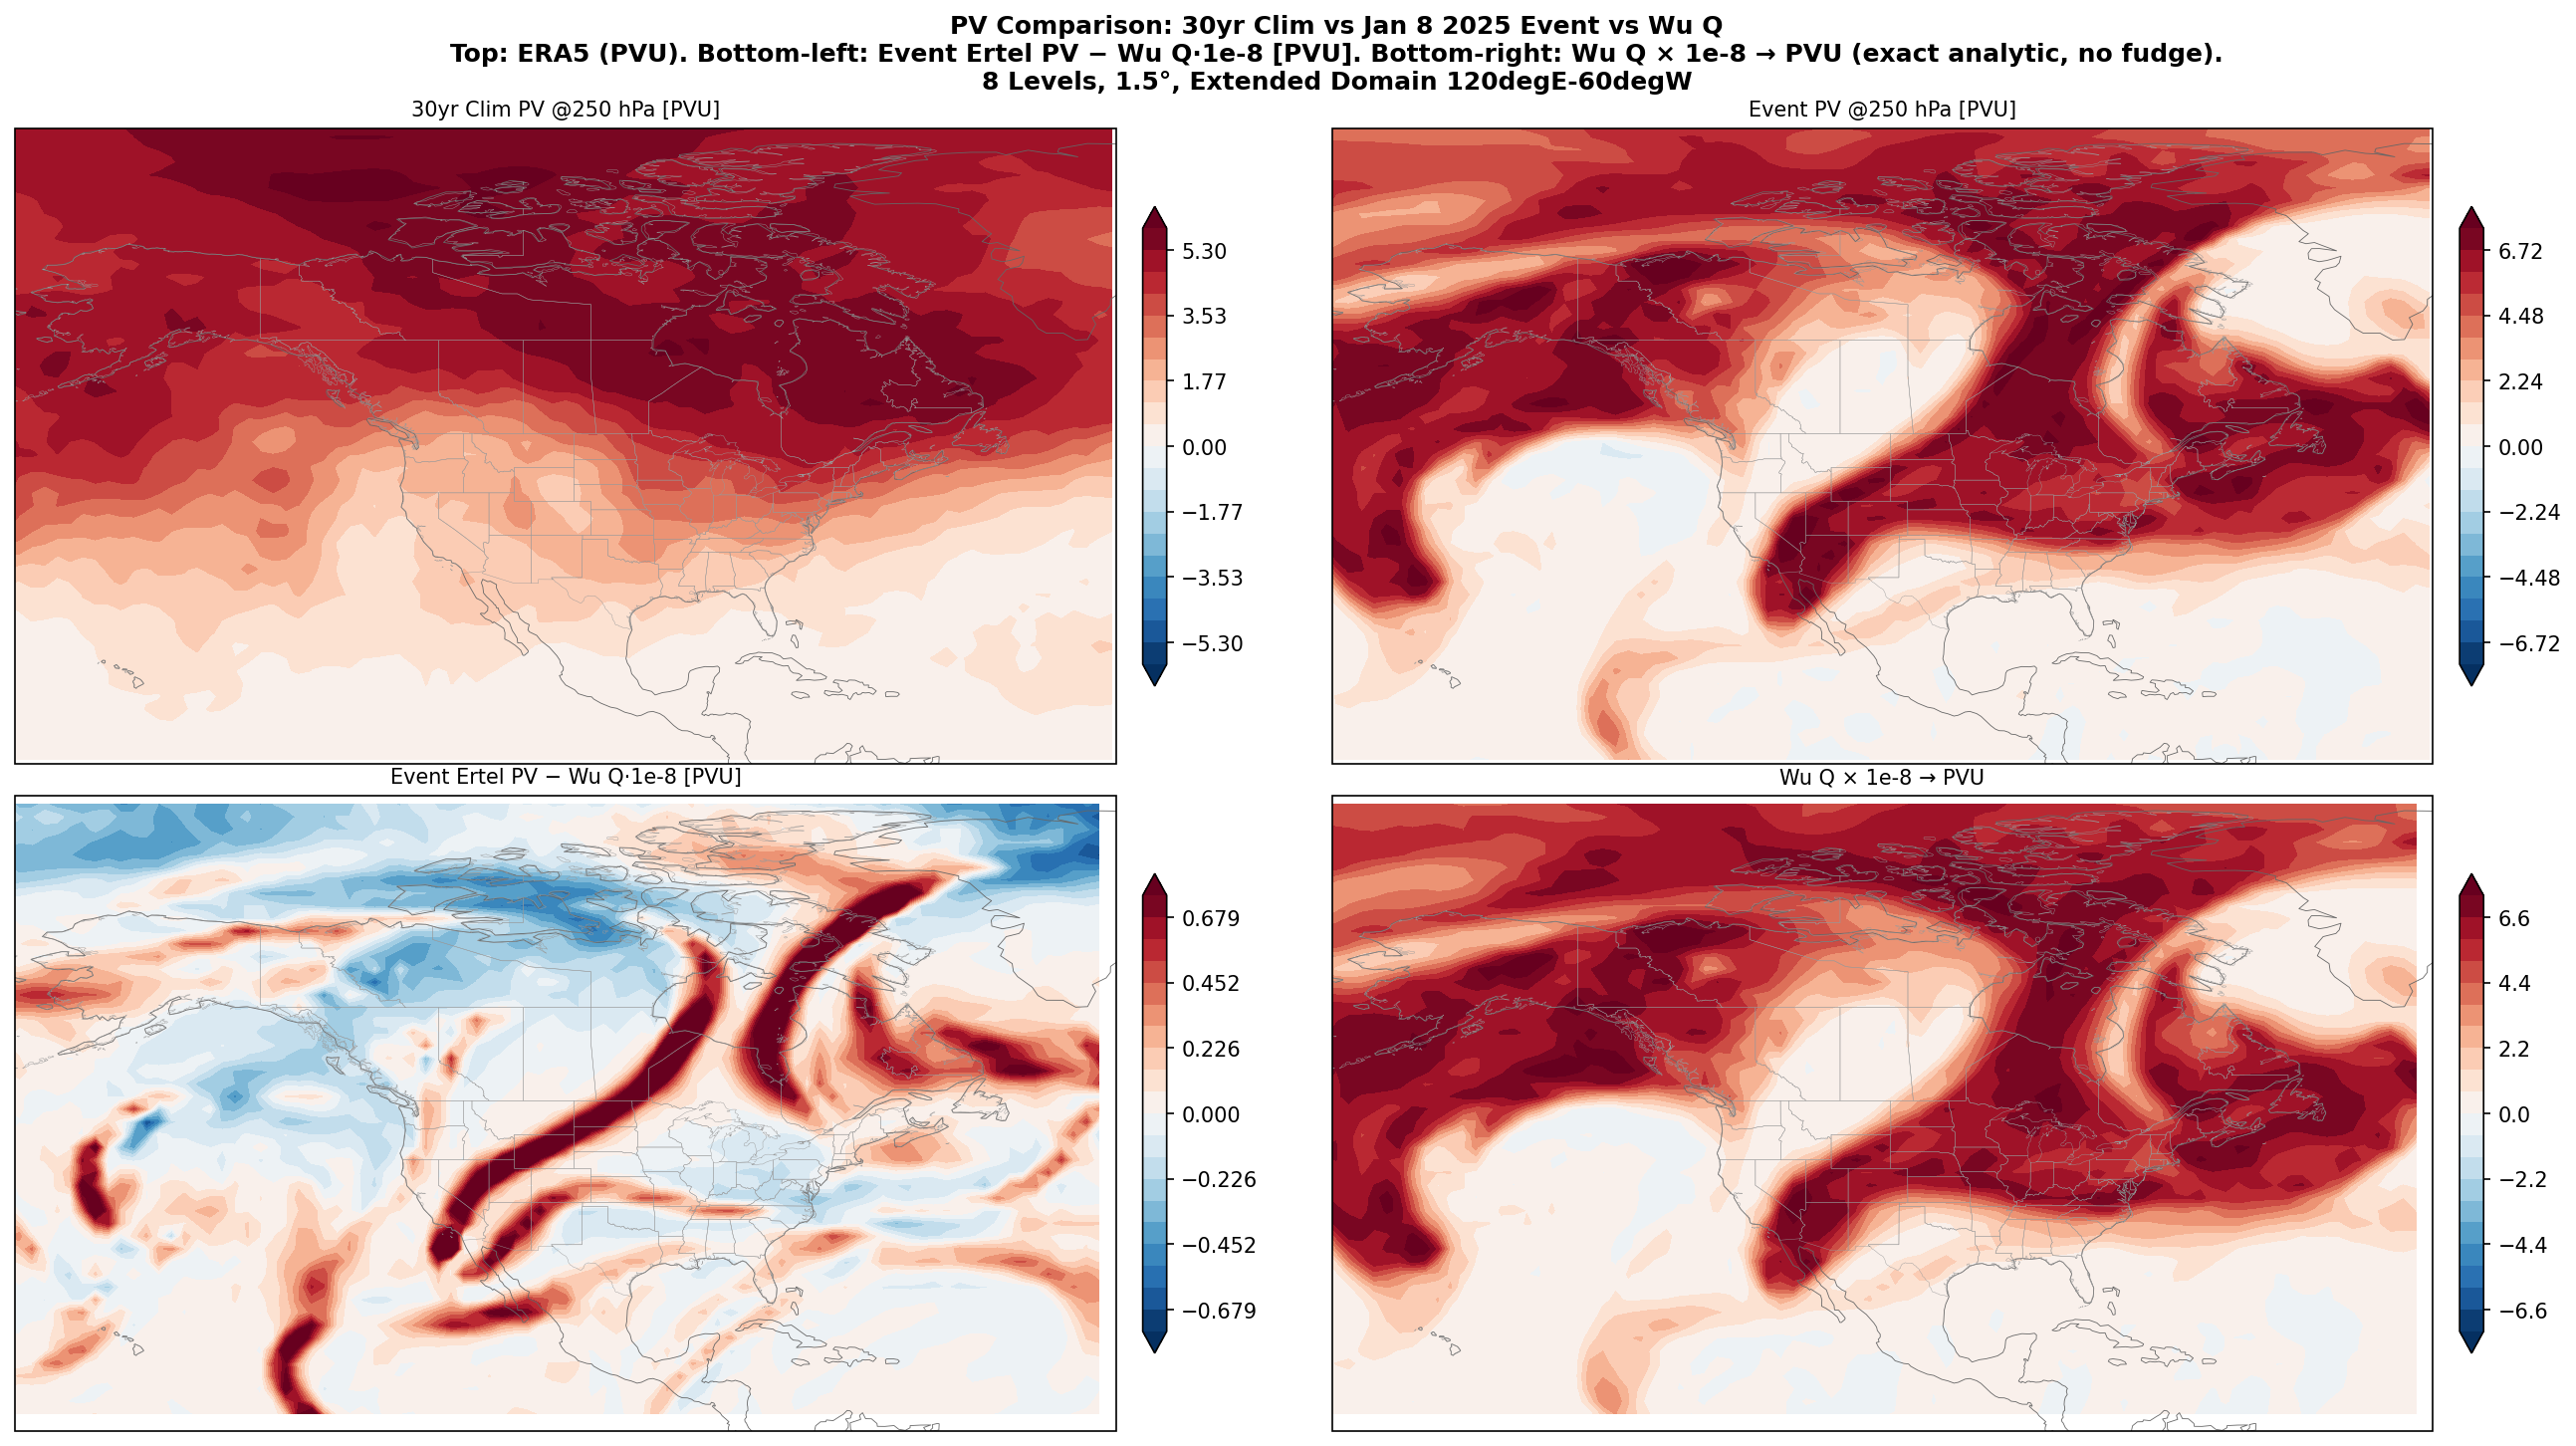
\includegraphics[width=0.85\textwidth]{figs/wu/pv_comparison_250hPa.png}
  \caption[Wu vs ERA5 PV]{\textbf{Step 08.} Wu $Q\times10^{-8}$ versus
  ERA5 native Ertel PV at $250$\,hPa.  After the raw-$T$ fix the median
  ratio is $1.00$ ($\corr=0.995$); no empirical scaling is used.}
  \label{fig:wu_vs_era5}
\end{figure}

\section{Step 10 --- Fig.~8 Replica (PV Advection)}
\label{sec:step10}

\begin{figure}[H]
  \centering
  
\includegraphics[width=0.92\textwidth]{figs/wu/fig8_replica.png}
  \caption[Davis 2022 Fig.~8 replica]{\textbf{Step 10.} Three-panel
  Davis-style PV-advection diagnostic, one panel per piece (surface /
  lower / upper): $250$\,hPa PV advection by the induced winds (fill),
  total PV anomaly (contours) and induced wind vectors (arrows).}
  \label{fig:wu_fig8}
\end{figure}

\section{Step 11 --- Cross-Sections and 3-D Structure}
\label{sec:step11}

Step~11 produces the latitude/longitude--pressure cross-sections and a
3-D ``vertical structure'' view, plus the linear-closure check.

\begin{figure}[H]
  \centering
  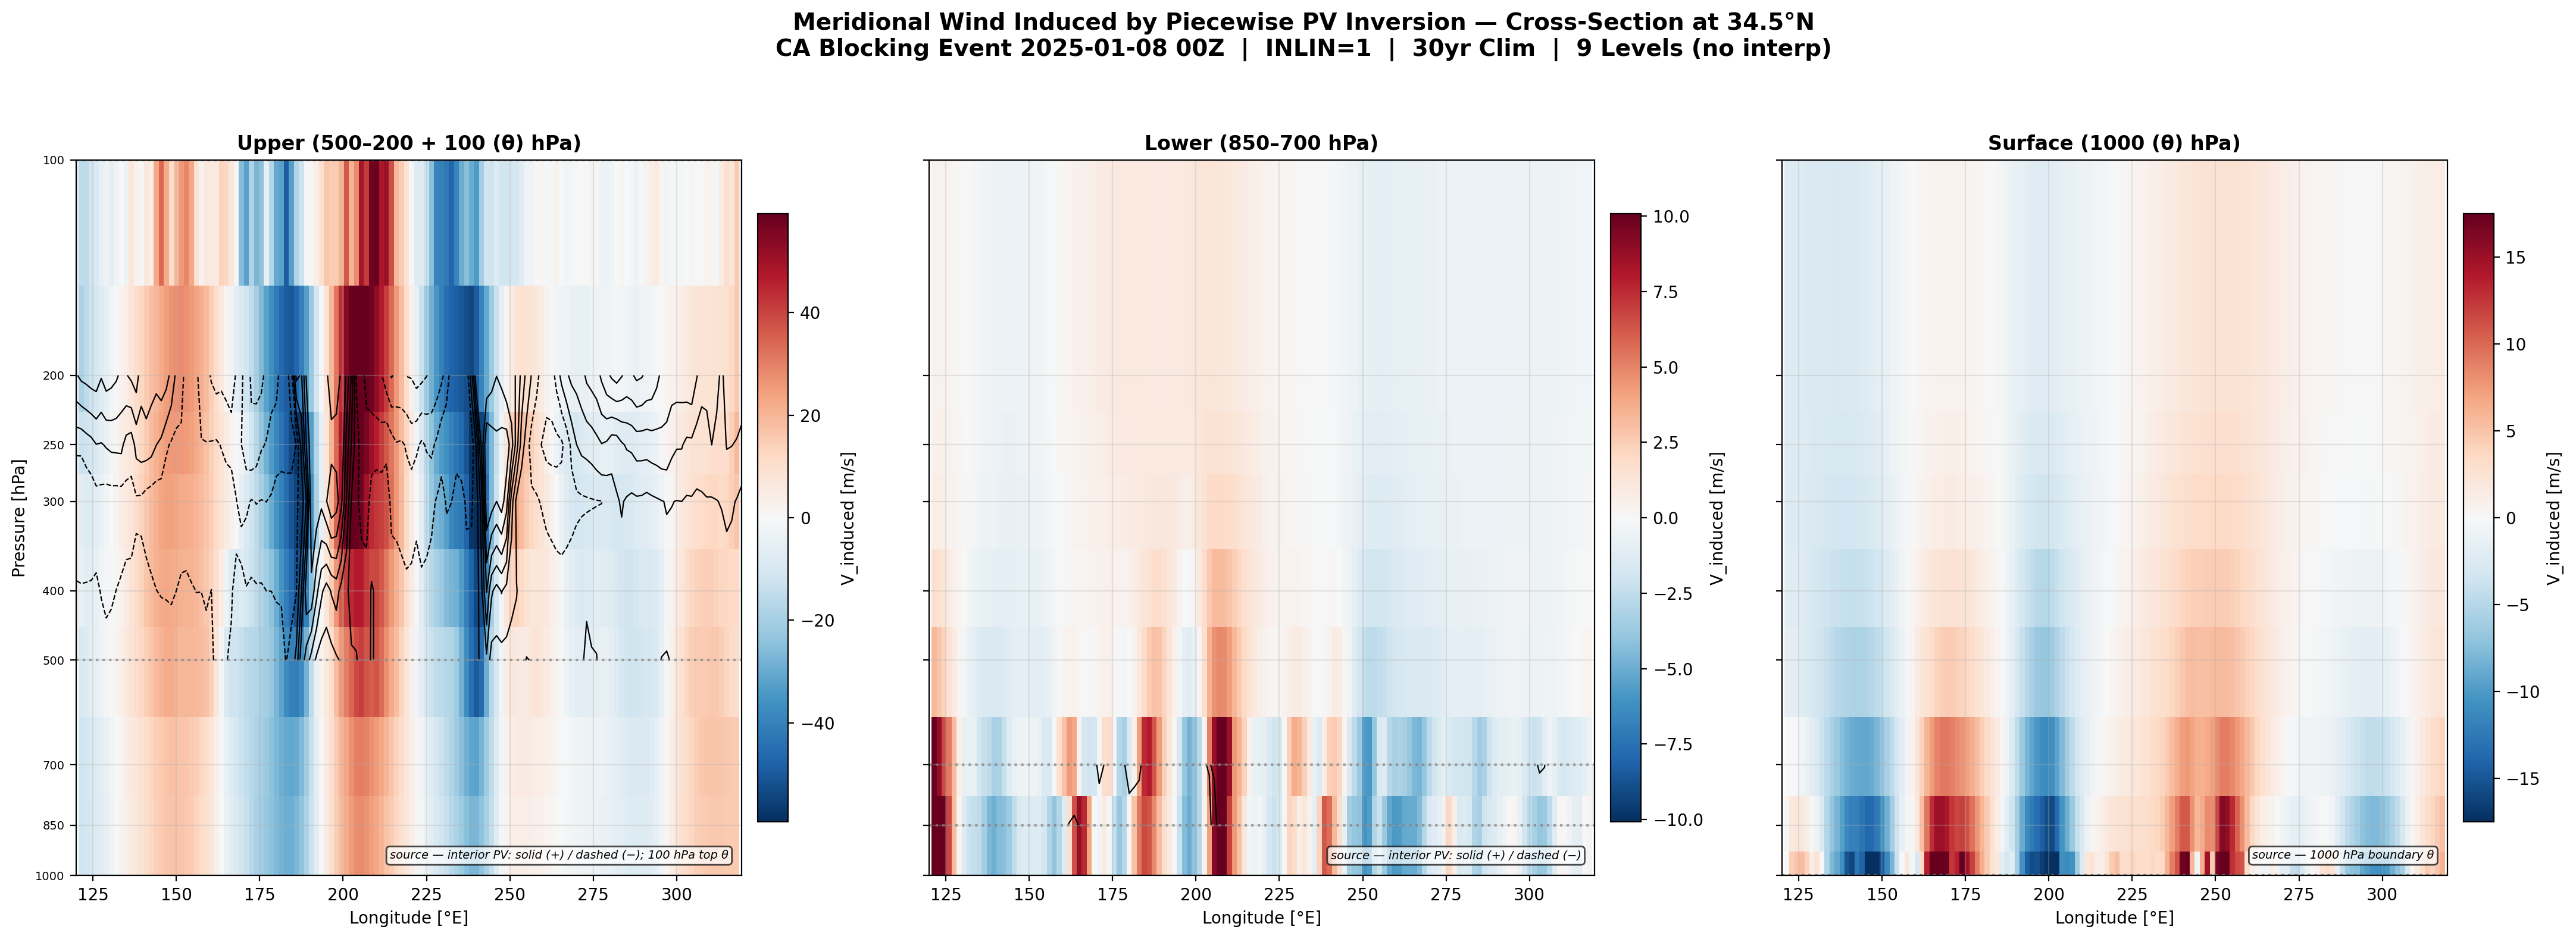
\includegraphics[width=\textwidth]{figs/wu/xsection_vinduced_3panel.png}
  \caption[Induced-wind cross-section]{\textbf{Step 11.} Zonal--vertical
  cross-section at $34.5^\circ$N of the meridional wind $v'$ induced by
  each piece, with each piece's \emph{own} source overlaid (interior PV
  contours; boundary-$\theta$ pieces labelled).  The \textbf{upper} piece
  peaks aloft ($\sim$250\,hPa, $\pm$50\,m\,s$^{-1}$); the \textbf{surface}
  piece is surface-trapped (peaks at 1000\,hPa, decaying upward) ---
  exactly the Bretherton boundary response.}
  \label{fig:wu_xsec}
\end{figure}

\begin{figure}[H]
  \centering
  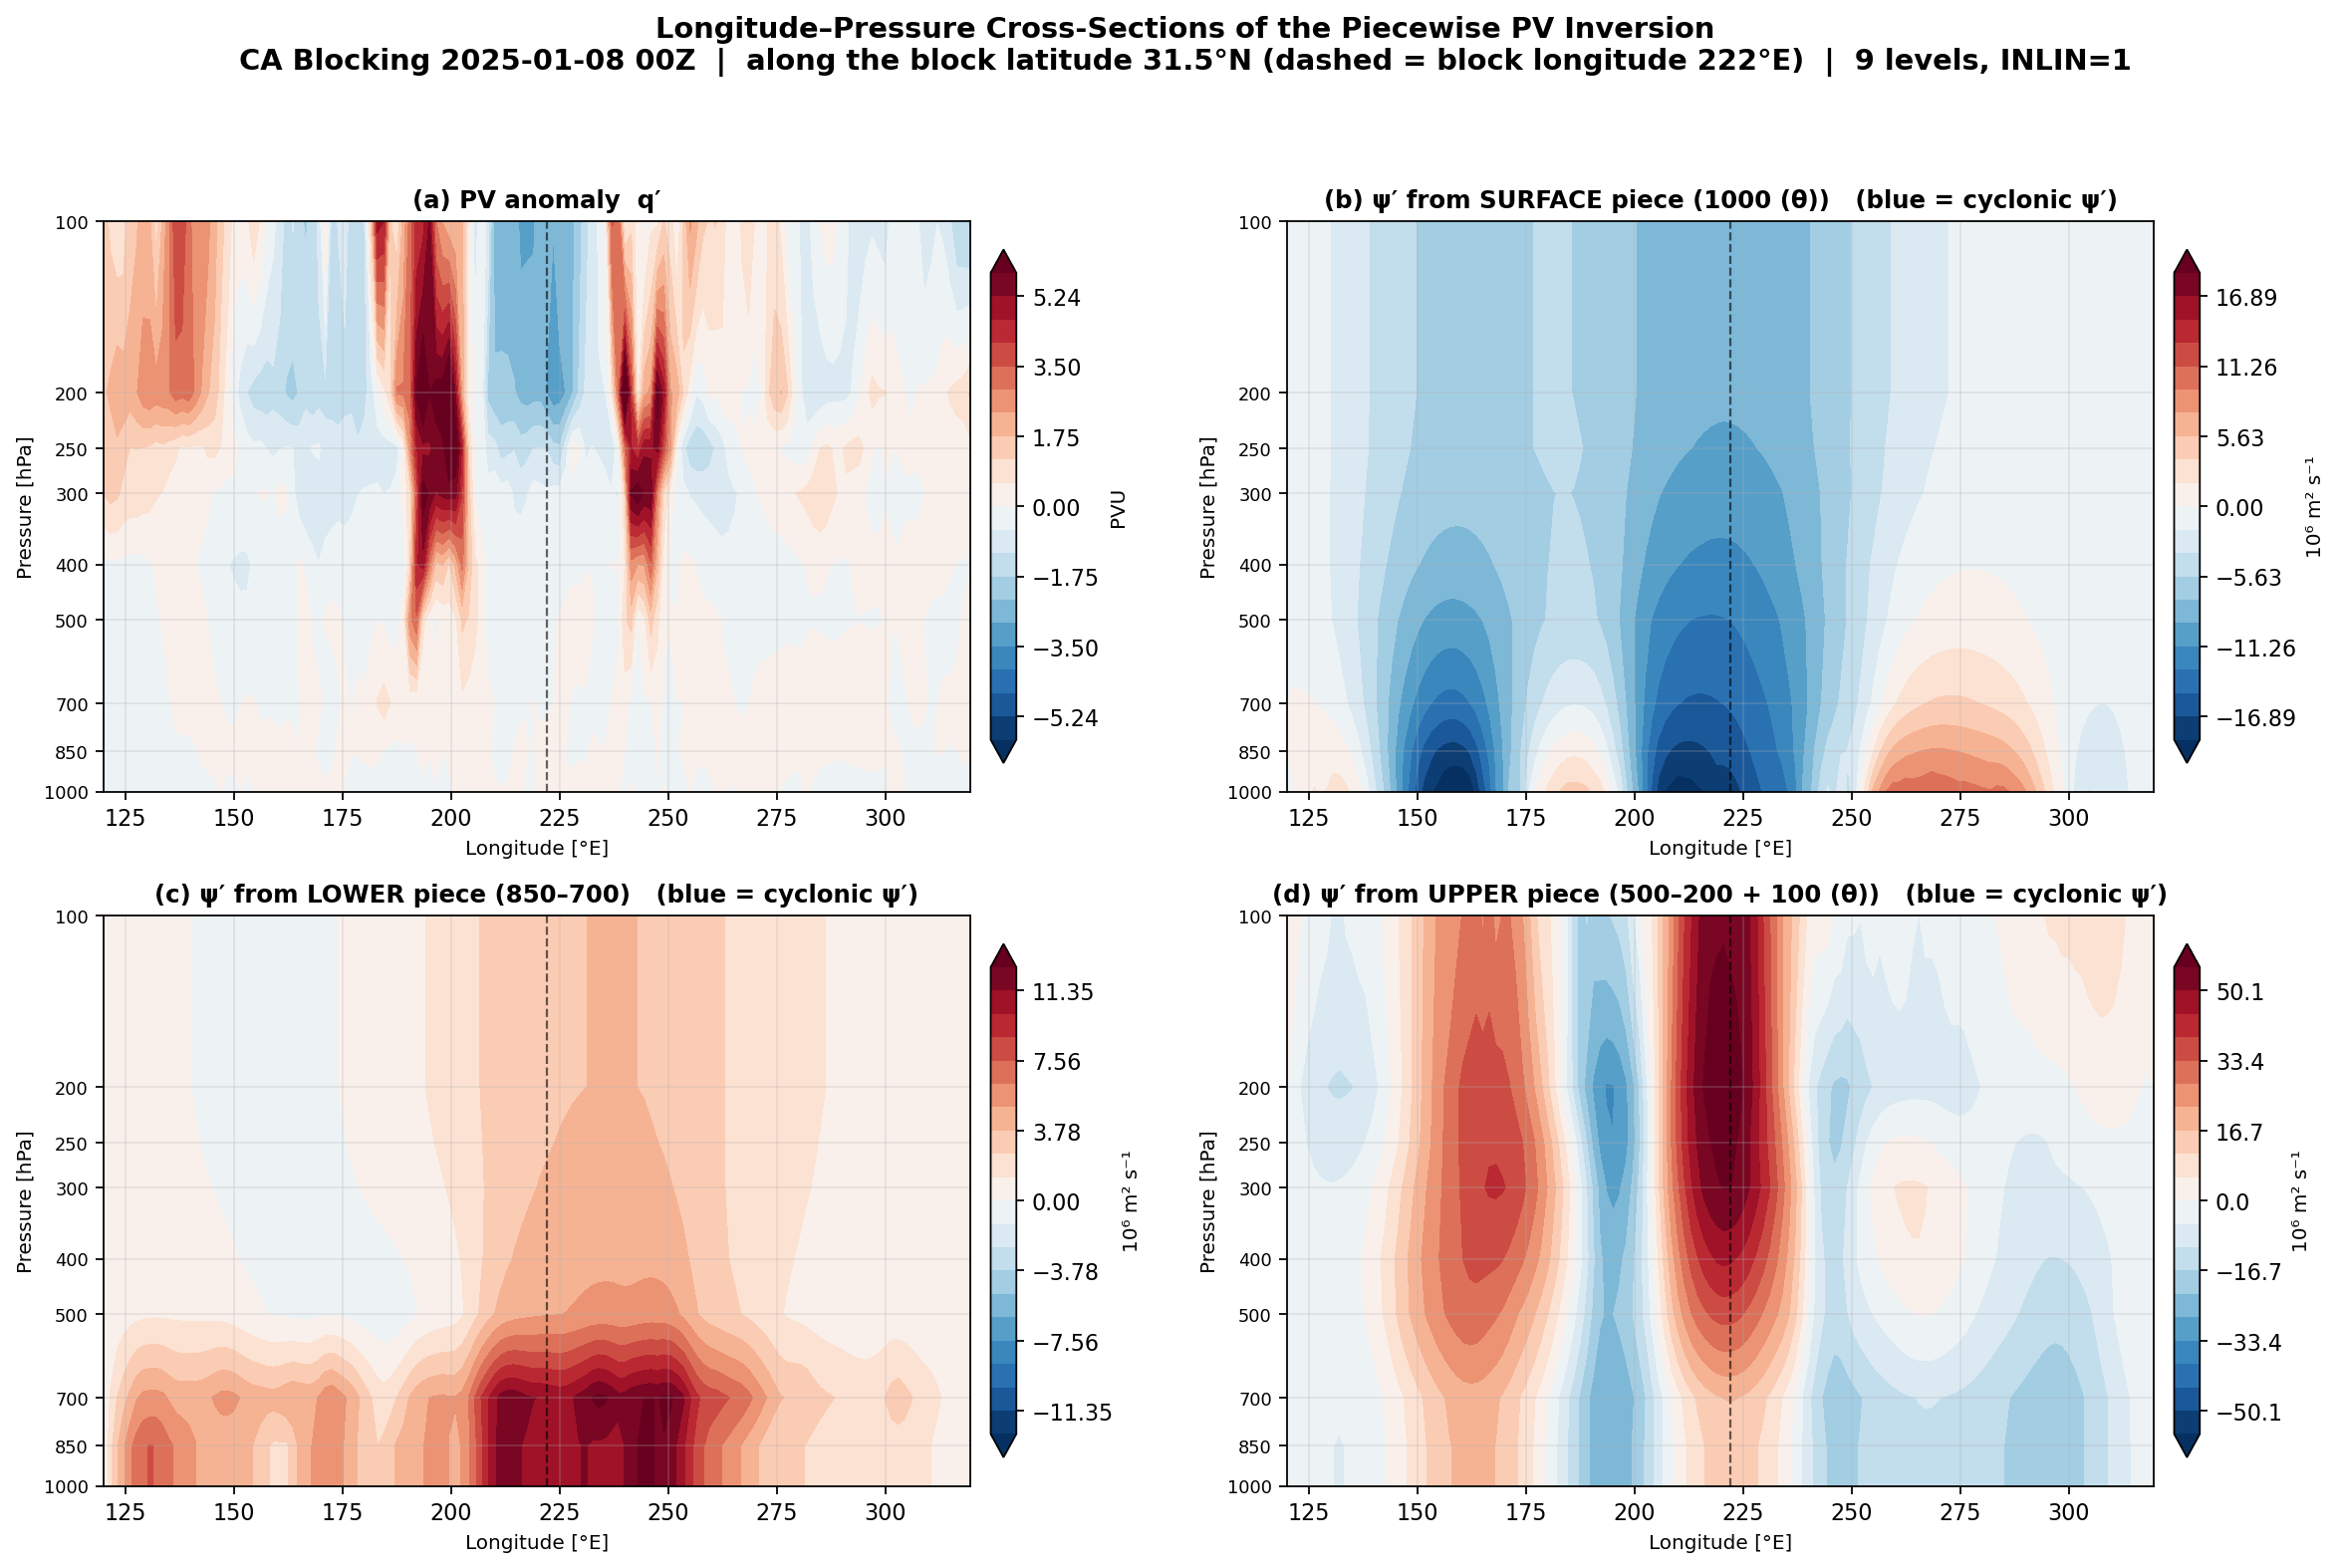
\includegraphics[width=\textwidth]{figs/wu/xsection_pv_psi_4panel.png}
  \caption[PV and piece-$\psi'$ cross-sections]{\textbf{Step 11.}
  Longitude--pressure ($x$--$p$) cross-sections at the block latitude
  ($31.5^\circ$N; dashed line $=$ block longitude $222^\circ$E):
  \textbf{(a)} total PV anomaly $q'$; \textbf{(b--d)} $\psi'$ induced by
  the surface, lower and upper pieces (blue $=$ cyclonic $\psi'<0$).  The
  PV anomaly is concentrated at upper levels (panel a); the surface
  boundary level carries no interior PV --- the surface heating is the
  boundary $\theta$ inverted in panel (b), a broad predominantly cyclonic
  response.  The upper piece (d) dominates the amplitude.}
  \label{fig:wu_3d}
\end{figure}

\begin{figure}[H]
  \centering
  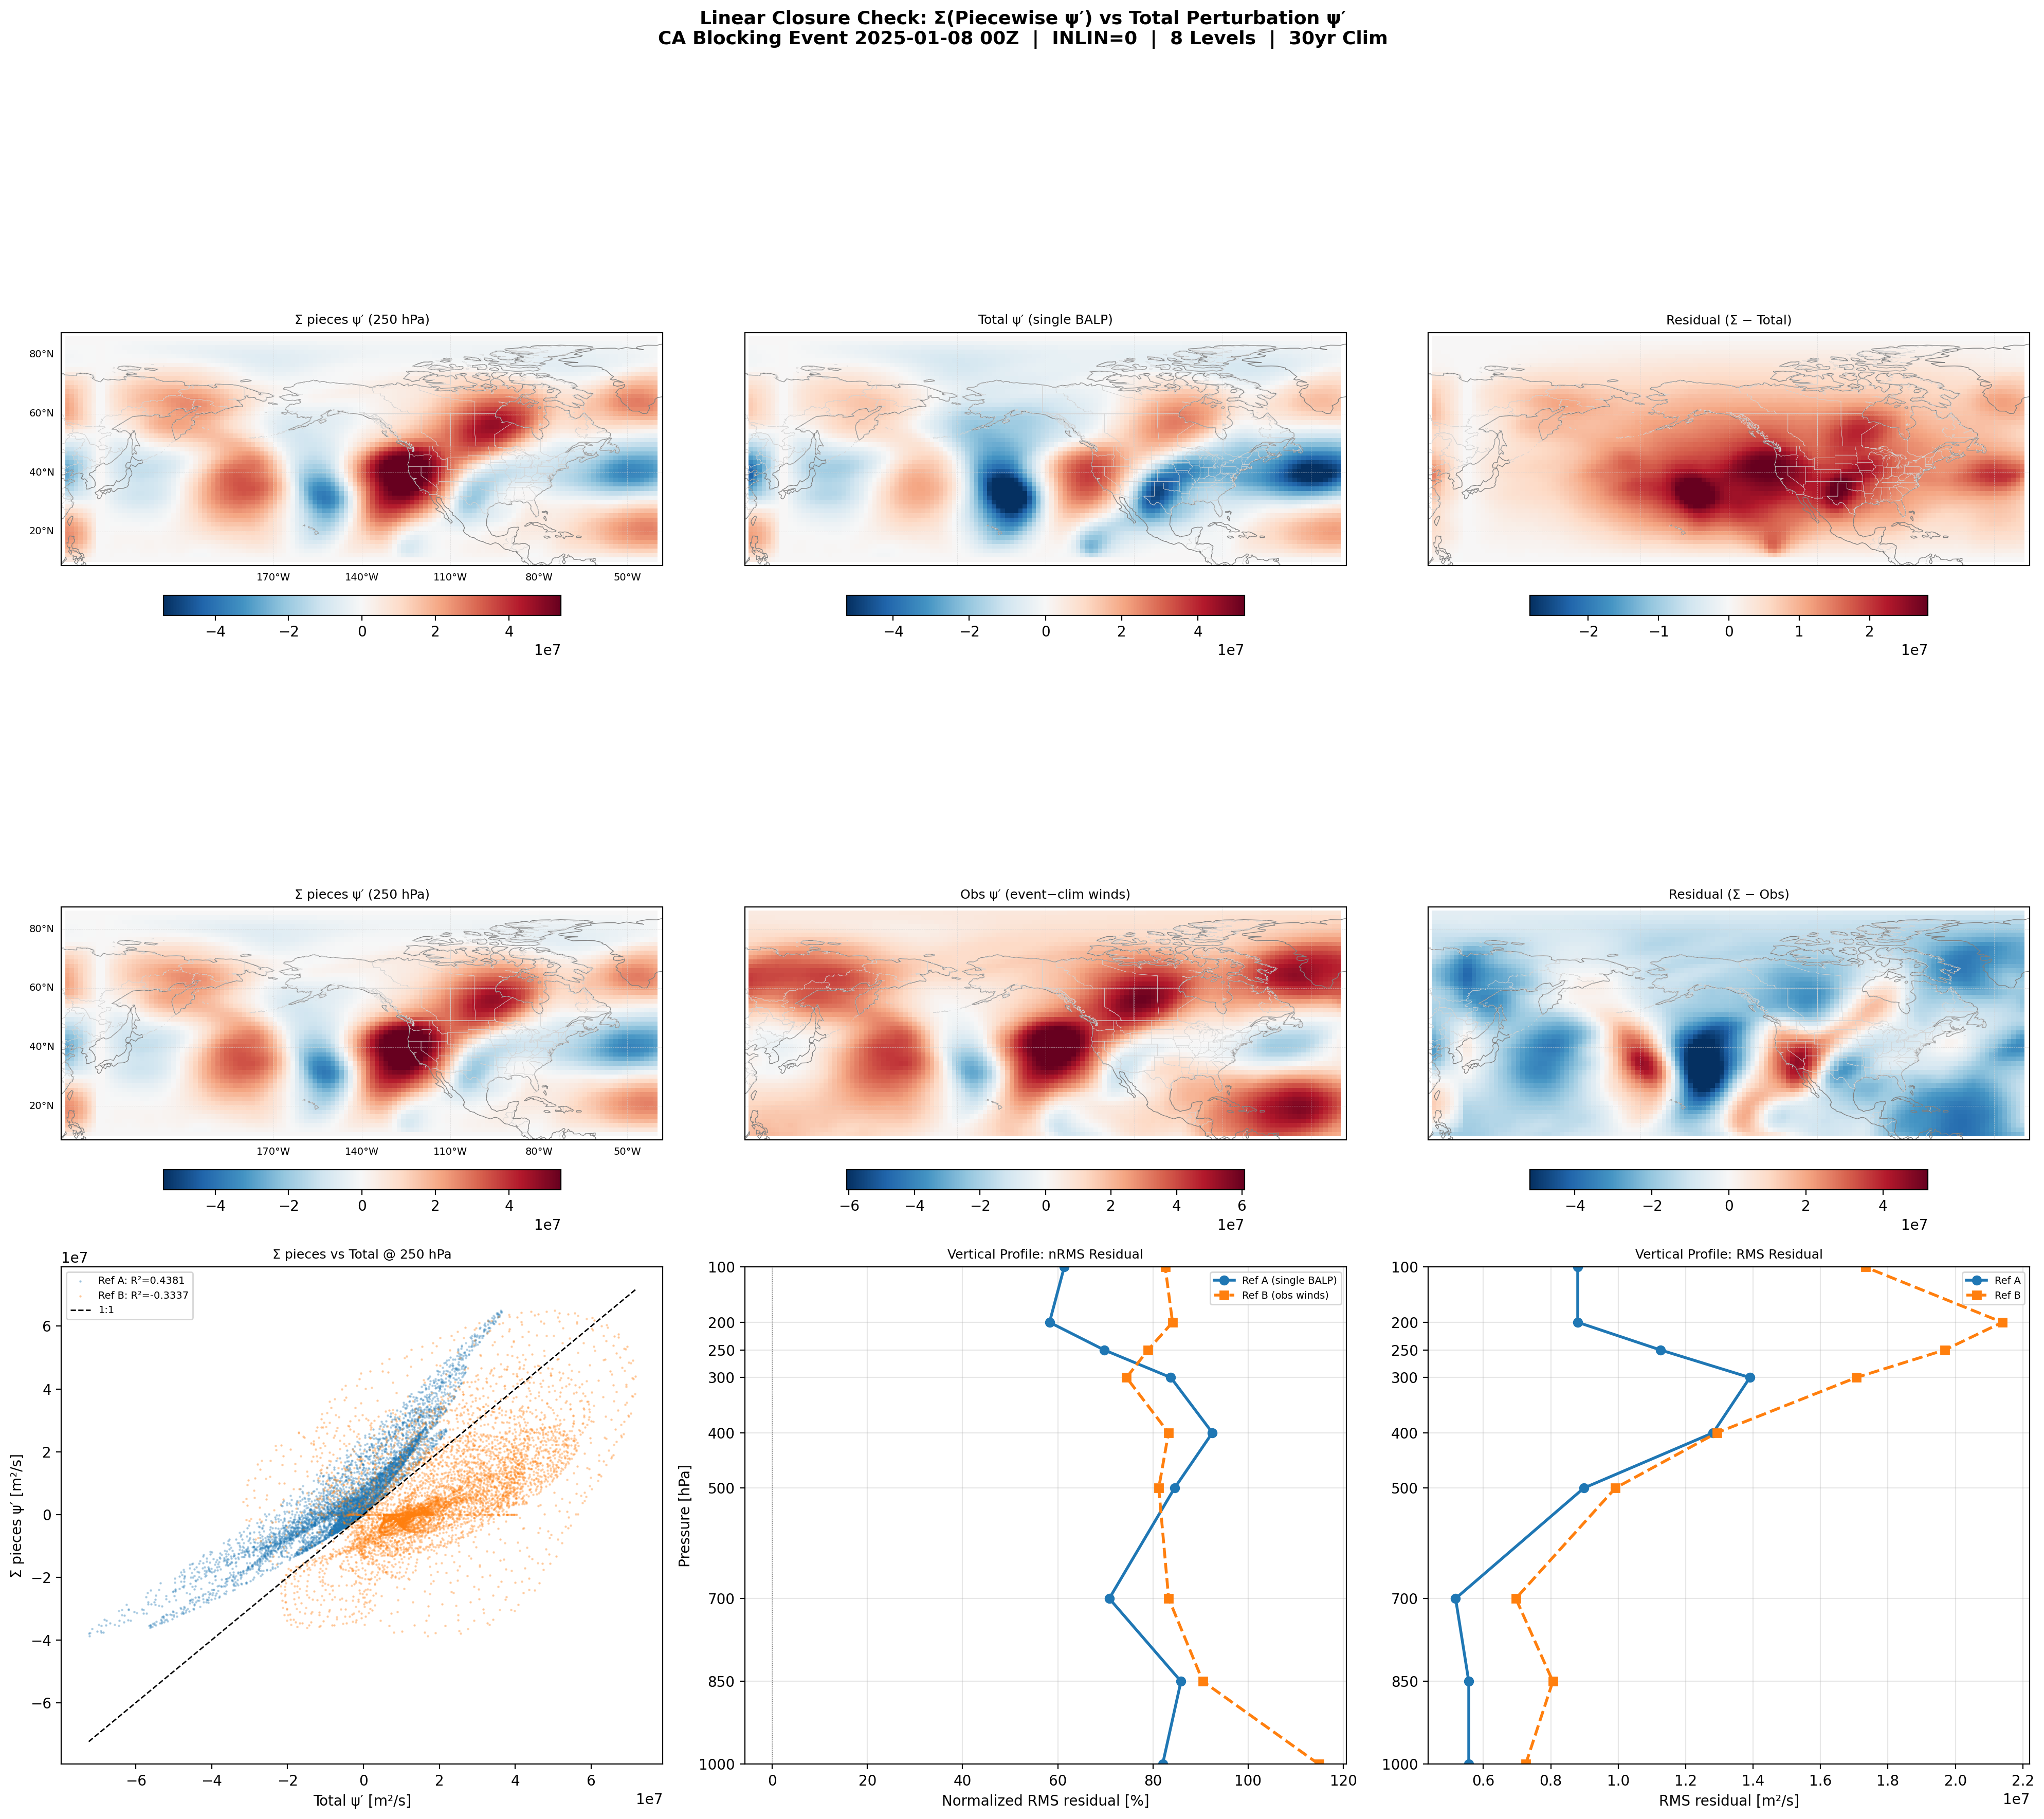
\includegraphics[width=0.95\textwidth]{figs/wu/closure_check.png}
  \caption[Linear closure check]{\textbf{Step 11.} Linear-closure check:
  the sum of the three piecewise $\psi'$ against a single all-levels
  inversion.  On the 9-level (top-100) grid the agreement is moderate
  ($R^2\!\approx\!0.44$ at 250\,hPa) --- a real grid effect, not a solver
  error (\Cref{sec:wu_converge}).}
  \label{fig:wu_closure}
\end{figure}
